\documentclass{article}
\usepackage{ae,aecompl}
\usepackage{todonotes}
\usepackage{chngcntr}
\usepackage{tikz-cd}
\usepackage{graphicx}
\graphicspath{ {./images/}}
\usepackage[all,cmtip]{xy}
\usepackage{amsmath, amscd}
\usepackage{amsthm}
\usepackage{amssymb}
\usepackage{amsfonts}
\usepackage{bm}
\usepackage{qsymbols}
\usepackage{latexsym}
\usepackage{mathrsfs}
\usepackage{mathtools}
\usepackage{cite}
\usepackage{color}
\usepackage{url}
\usepackage{enumerate}
\usepackage{verbatim}
\usepackage[draft=false, colorlinks=true]{hyperref}
\usepackage{pdfpages}
\usepackage[margin=1.2in]{geometry}
\usepackage{IEEEtrantools}

\usepackage{fancyhdr}


\usepackage[nameinlink]{cleveref}


\DeclareMathOperator*{\ac}{accept}
\DeclareMathOperator*{\amax}{argmax}
\DeclareMathOperator*{\amin}{argmin}
\DeclareMathOperator*{\Aut}{Aut}
\newcommand {\al}{{\alpha}}
\newcommand {\abs}[1]{{\left\lvert#1\right\rvert}}
\newcommand {\A}{{\mathcal{A}}}
\newcommand {\AM}{{\mathrm{AM}}}
\newcommand {\AMp}{{\AM_{p}^{X}\!(\Ri_\w)}}
\newcommand {\B}{{\mathcal{B}}}
\DeclareMathOperator*{\Be}{Bern}
\newcommand {\Br}{{\dot{B}}}
\newcommand {\Ba}{{\mathfrak{B}}}
\newcommand {\C}{{\mathbb C}}
\newcommand {\ce}{\mathrm{c}}
\newcommand {\Ce}{\mathrm{C}}
\newcommand {\Cc}{\mathrm{C_{c}}}
\newcommand {\Ccinf}{\mathrm{C_{c}^{\infty}}}
\DeclareMathOperator{\cov}{Cov}
\DeclareMathOperator{\DEV}{DEV}
\newcommand {\Di}{{\mathbb D}}
\newcommand {\dom}{\mathrm{dom}}
\newcommand{\dist}{\stackrel{\mathrm{dist}}{=}}
\newcommand {\ud}{\mathrm{d}}
\newcommand {\ue}{\mathrm{e}}
\newcommand {\eps}{\varepsilon}
\newcommand {\veps}{\varepsilon}
\newcommand {\vrho}{{\varrho}}
\newcommand {\E}{{\mathbb{E}}}
\newcommand {\Ec}{{\mathcal{E}}}
\newcommand {\Ell}{L}
\newcommand {\Ellp}{{L_{p}[0,1]}}
\newcommand {\Ellpprime}{{L_{p'}([0,1])}}
\newcommand {\Ellq}{{L_{q}([0,1])}}
\newcommand {\Ellqprime}{{L_{q'}([0,1])}}
\newcommand {\Ellr}{L^{r}}
\newcommand {\Ellone}{{L_{1}([0,1])}}
\newcommand{\Elltwo}{{L_{2}([0,1])}}
\newcommand{\Ellinfty}{L^{\infty}}
\newcommand{\Ellinftyc}{L_{\mathrm{c}}^{\infty}}
\newcommand{\exb}[1]{\exp\left\{#1\right\}}
\DeclareMathOperator*{\Ext}{Ext}
\newcommand{\F}{{\mathcal{F}}}
\newcommand{\Fe}{{\mathbb{F}}}
\newcommand{\G}{{\mathcal{G}}}
\newcommand{\HF}{\mathcal{H}_{\text{FIO}}^{1}(\Rd)}
\newcommand{\Hr}{H}
\newcommand{\HT}{\mathcal{H}}
\newcommand{\ui}{\mathrm{i}}
\newcommand{\I}{{I}}
\newcommand{\J}{{\mathcal{J}}}
\newcommand{\id}{{\mathrm{id}}}
\newcommand{\iid}{\stackrel{\mathclap{\normalfont\mbox{iid}}}{\sim}}
\newcommand{\im}{{\text{im }}}
\newcommand{\ind}{{\perp\!\!\!\perp}}
\DeclareMathOperator*{\Int}{int}
\newcommand{\intx}{{\overline{\int_{X}}}}
\newcommand{\inte}{{\overline{\int_{\E}}}}
\newcommand{\la}{\lambda}
\newcommand{\rb}{\rangle}
\newcommand{\lb}{{\langle}}
\newcommand{\La}{\Lambda}
\newcommand{\calL}{{\mathcal{L}}}
\newcommand{\lp}{{\mathcal{L}}^{p}}
\newcommand{\lpo}{{\overline{\mathcal{L}}^{p}\!}}
\newcommand{\Lpo}{{\overline{\Ell}^{p}\!}}
\newcommand{\M}{{\mathbf{M}}}
\newcommand{\Ma}{{\mathcal{M}}}
\newcommand{\N}{{{\mathbb N}}}
\newcommand{\Na}{{{\mathcal{N}}}}
\newcommand{\norm}[1]{\left\|#1\right\|}
\newcommand{\normm}[1]{{\left\vert\kern-0.25ex\left\vert\kern-0.25ex\left\vert #1 
    \right\vert\kern-0.25ex\right\vert\kern-0.25ex\right\vert}}
\newcommand{\Om}{{{\Omega}}}
\newcommand{\one}{{{\bf 1}}}
\newcommand{\pic}{\text{Pic }}
\newcommand{\ph}{{\varphi}}
\newcommand{\Pa}{{\mathbb{P}}}
\newcommand{\Po}{{\mathcal{P}}}
\newcommand{\Q}{{\mathbb{Q}}}
\newcommand{\R}{{\mathbb R}}
\newcommand{\Rd}{{\mathbb{R}^{d}}}
\DeclareMathOperator{\rej}{reject }
\newcommand{\Rn}{{\mathbb{R}^{n}}}
\newcommand{\cR}{{\mathcal{R}}}
\newcommand{\Rad}{{\mathrm{Rad}}}
\newcommand{\ran}{{\mathrm{ran}}}
\newcommand{\Ri}{{\mathrm{R}}}
\newcommand{\supp}{{\mathrm{supp}}}
\newcommand{\Se}{\mathrm{S}}
\newcommand{\Sp}{S^{*}(\Rn)}
\newcommand{\St}{{\mathrm{St}}}
\newcommand{\Sw}{\mathcal{S}}
\newcommand{\T}{{\mathcal{T}}}
\newcommand{\ta}{{\theta}}
\newcommand{\Ta}{{\Theta}}
\newcommand{\topp}{\stackrel{p}{\to}}
\newcommand{\todd}{\stackrel{d}{\to}}
\newcommand{\toL}[1]{\stackrel{L^{#1}}{\to}} 
\newcommand{\toas}{\stackrel{a.s.}{\to}}
\DeclareMathOperator{\V}{Var}
\newcommand {\w}{{\omega}}
\newcommand {\W}{{\mathrm{W}}}
\newcommand {\Wnp}{\text{$\mathrm{W}$\textsuperscript{$n,\!p$}}}
\newcommand {\Wnpeq}{\text{$\mathrm{W}$\textsuperscript{$n\!,\!p$}}}
\newcommand {\Wonep}{\text{$\mathrm{W}$\textsuperscript{$1,\!p$}}}
\newcommand {\Wonepeq}{\text{$\mathrm{W}$\textsuperscript{$1\!,\!p$}}}
\newcommand {\X}{{\mathcal{X}}}
\newcommand {\Z}{{{\mathbb Z}}}
\newcommand {\Za}{{\mathcal{Z}}}
\newcommand {\Zd}{{\Z[\sqrt{d}]}}
\newcommand {\vanish}[1]{\relax}

\newcommand {\wh}{\widehat}
\newcommand {\wt}{\widetilde}
\newcommand {\red}{\color{red}}

% Distributions
\newcommand{\normal}{\mathsf{N}}
\newcommand{\poi}{\mathsf{Poisson}}
\newcommand{\bern}{\mathsf{Bernoulli}}
\newcommand{\bin}{\mathsf{Binomal}}
\newcommand{\multi}{\mathsf{Multinomial}}
\newcommand{\Exp}{\mathsf{Exp}}



% put your command and environment definitions here




% some theorem environments
% remove "[theorem]" if you do not want them to use the same number sequence


  \newtheorem{thrm}{Theorem}
  \newtheorem{lemma}{Lemma}
  \newtheorem{prop}{Proposition}
  \newtheorem{cor}{Corollary}

  \newtheorem{conj}{Conjecture}
  \renewcommand{\theconj}{\Alph{conj}}  % numbered A, B, C etc

  \theoremstyle{definition}
  \newtheorem{defn}{Definition}
  \newtheorem{ex}{Example}
  \newtheorem{exs}{Examples}
  \newtheorem{question}{Question}
  \newtheorem{remark}{Remark}
  \newtheorem{notn}{Notation}
  \newtheorem{exer}{Exercise}




\title{STATS305A - Lecture 11}
\author{John Duchi\\ Scribed by Michael Howes}
\date{10/26/21}

\pagestyle{fancy}
\fancyhf{}
\rhead{STATS305A - Lecture 11}
\lhead{10/26/21}
\rfoot{Page \thepage}

\begin{document}
\maketitle
\tableofcontents
\section{Announcements}
\begin{itemize}
    \item Homework 2 due today.
    \item Etude 2 due on Thursday.
\end{itemize}
\section{Leverage}
In the linear model $Y = X\beta+\eps$, we define $H=X(X^TX)^{-1}X^T$ and we define 
\[H_{ii} = i^{th} \text{ diagonal entry of }H = i^{th} \text{ leverage score}. \]
We have seen multiple interpretations of leverage score:
\begin{itemize}
    \item Self influence of example $i$ on itself.
    \item $\frac{\partial \wh{y}_i}{\partial y_i} = H_{ii}$.
\end{itemize}
We also have the leave one out calculation. We saw that if $\wh{y}_{\setminus i} = x_i^T\wh{\beta}_{\setminus j}$ where $\wh{\beta}_{\setminus i} = (X_{\setminus i}^TX_{\setminus i})^{-1}X^T_{\setminus i}Y_{\setminus i}$ and
\[X_{\setminus i}=[x_j^T]_{j\neq i} \in \R^{(n-1)\times d} ~~ \text{and}~~ Y_{\setminus i} = [Y_j]_{j\neq i} \in \R^{n-1}, \]
then 
\[\wh{y}_i = x_i^T\wh{\beta} = (1-H_{ii})\wh{y}_{\setminus i}+H_{ii}y_i. \]
Thus (since $H_{ii}\in [0,1]$), $\wh{y}_i$ is a convex combination of $\wh{y}_{\setminus i}$ and $y_i$. This also gives us a way to effeciently calculate every $\wh{y}_{\setminus i}$. This is something special about the linear model. Note that if we rearrange the above expression we get
\[\wh{y}_{\setminus i} = \frac{1}{1-H_{ii}}\wh{y}_i - \frac{H_{ii}}{1-H_{ii}}y_i, \]
Thus
\[[\wh{y}_{\setminus i}]_{i=1}^n = \diag(I-H)^{-1}\left(\wh{y}-\diag(H)y\right).  \]
Thus in $O(n)$ times we can do \emph{all} leave one out predictions assuming that we have the matrix $H$.

\section{Residuals, variance and leverage score}
Recall $\wh{\eps} = Y-\wh{Y} = (I-H)Y$. We always have $\wh{\eps}^T\wh{Y}=0$. This is because
\[\wh{\eps}^T\wh{Y} = \wh{Y}^T(I-H)H\wh{Y} = \wh{Y}^T(H-H)\wh{Y}=0. \]
The intepretation is that $\wh{\eps}$ is the noise after removing all ``information'' in the directions of $\range(X)$ and $\wh{Y}$ is the expected value of $Y$ in the $X$ directions.

Now suppose we have the distributional assumptions $Y=X\beta+\eps$ where $\eps \sim (0,\sigma^2I)$. We then have $\wh{\eps} \sim (0,\sigma^2(I-H))$ and so
\[\text{cov}(\wh{\eps}_i,\wh{\eps}_j) = \begin{cases}
    \sigma^2(1-H_{ii}) & \text{if } i=j,\\
    -\sigma^2H_{ij} & \text{else}.
\end{cases} \]
And
\[\text{Cov}(\wh{y},\wh{\eps}) = 0.\] 
Thus the residuals are typically correlated even when have noise $\eps \sim (0,\sigma^2 I)$ (in this case we say that the noise is \emph{homoscedastic}). Note also that
\[\V(\wh{\eps}_i) = \sigma^2(1-H_{ii}) \le \sigma^2 = \V(\eps_i). \]
We call the above decrease in variance, \emph{variance deflation}. The larger the leverage score, the more deflation we have. 

Recall the below picture and our intuition that a point with high leverage may be problematic and that the high leverage points are characterized by $x_{i}$ being far from the ``bulk'' of $X$. If we have a point of high leverage $x_i$, then we could imagine two worlds with different values of $y_i$. Since $x_i$ is high leverage, the point $\wh{y}_i = x_i^T \wh{\beta}$ changes a lot as $y_i$ changes. This means that our model is more sensitive to changes in $y_i$ than changes in $y$ at points with low leverage.

\begin{center}
    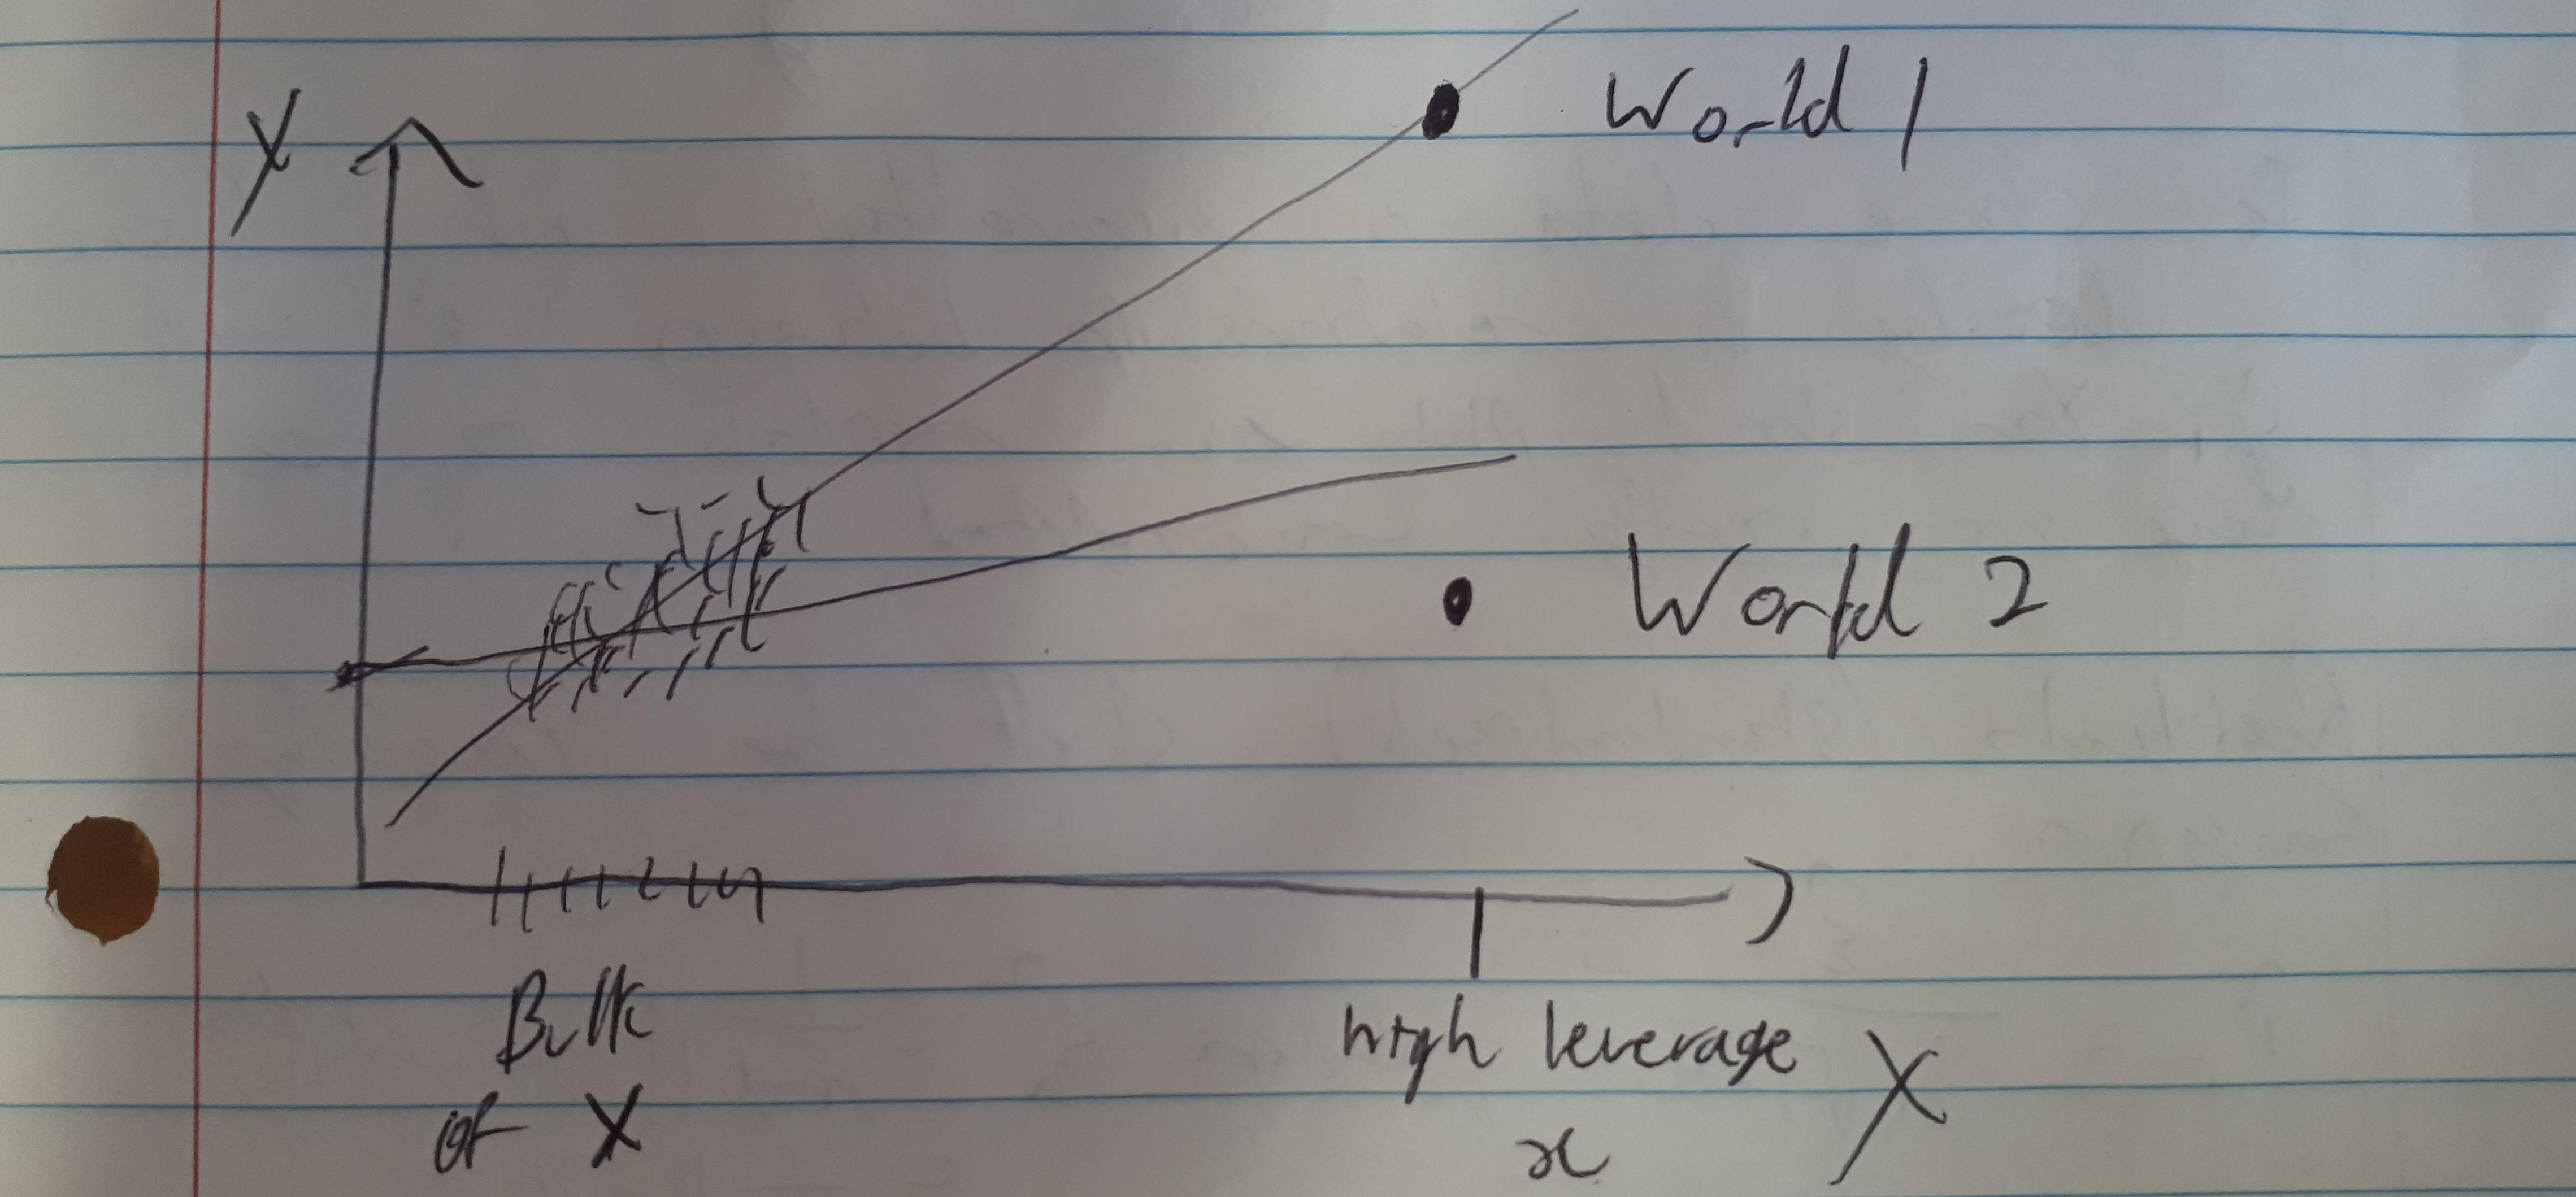
\includegraphics[width = \textwidth/2]{10_26_P01.jpg}
\end{center}

\section{Plots and diagnostics}
How do we decide if our linear models are ``good enough''? We have a number of \underline{possible desiderata}. Some plots which are good sanity checkes
\begin{itemize}
    \item Residuals vs fitted values.
    \item Residuals vs individual features ie columns in $X$.
    \item Residuals vs quantiles of Gaussians called a QQ or quantile quantile plot.
\end{itemize}

\subsection{Residuals vs predicted values}
One is that the residual $\wh{\eps}$ should be \emph{really} uncorrelated with the predicted values $\wh{y}$. Consider the below plot:

\begin{center}
    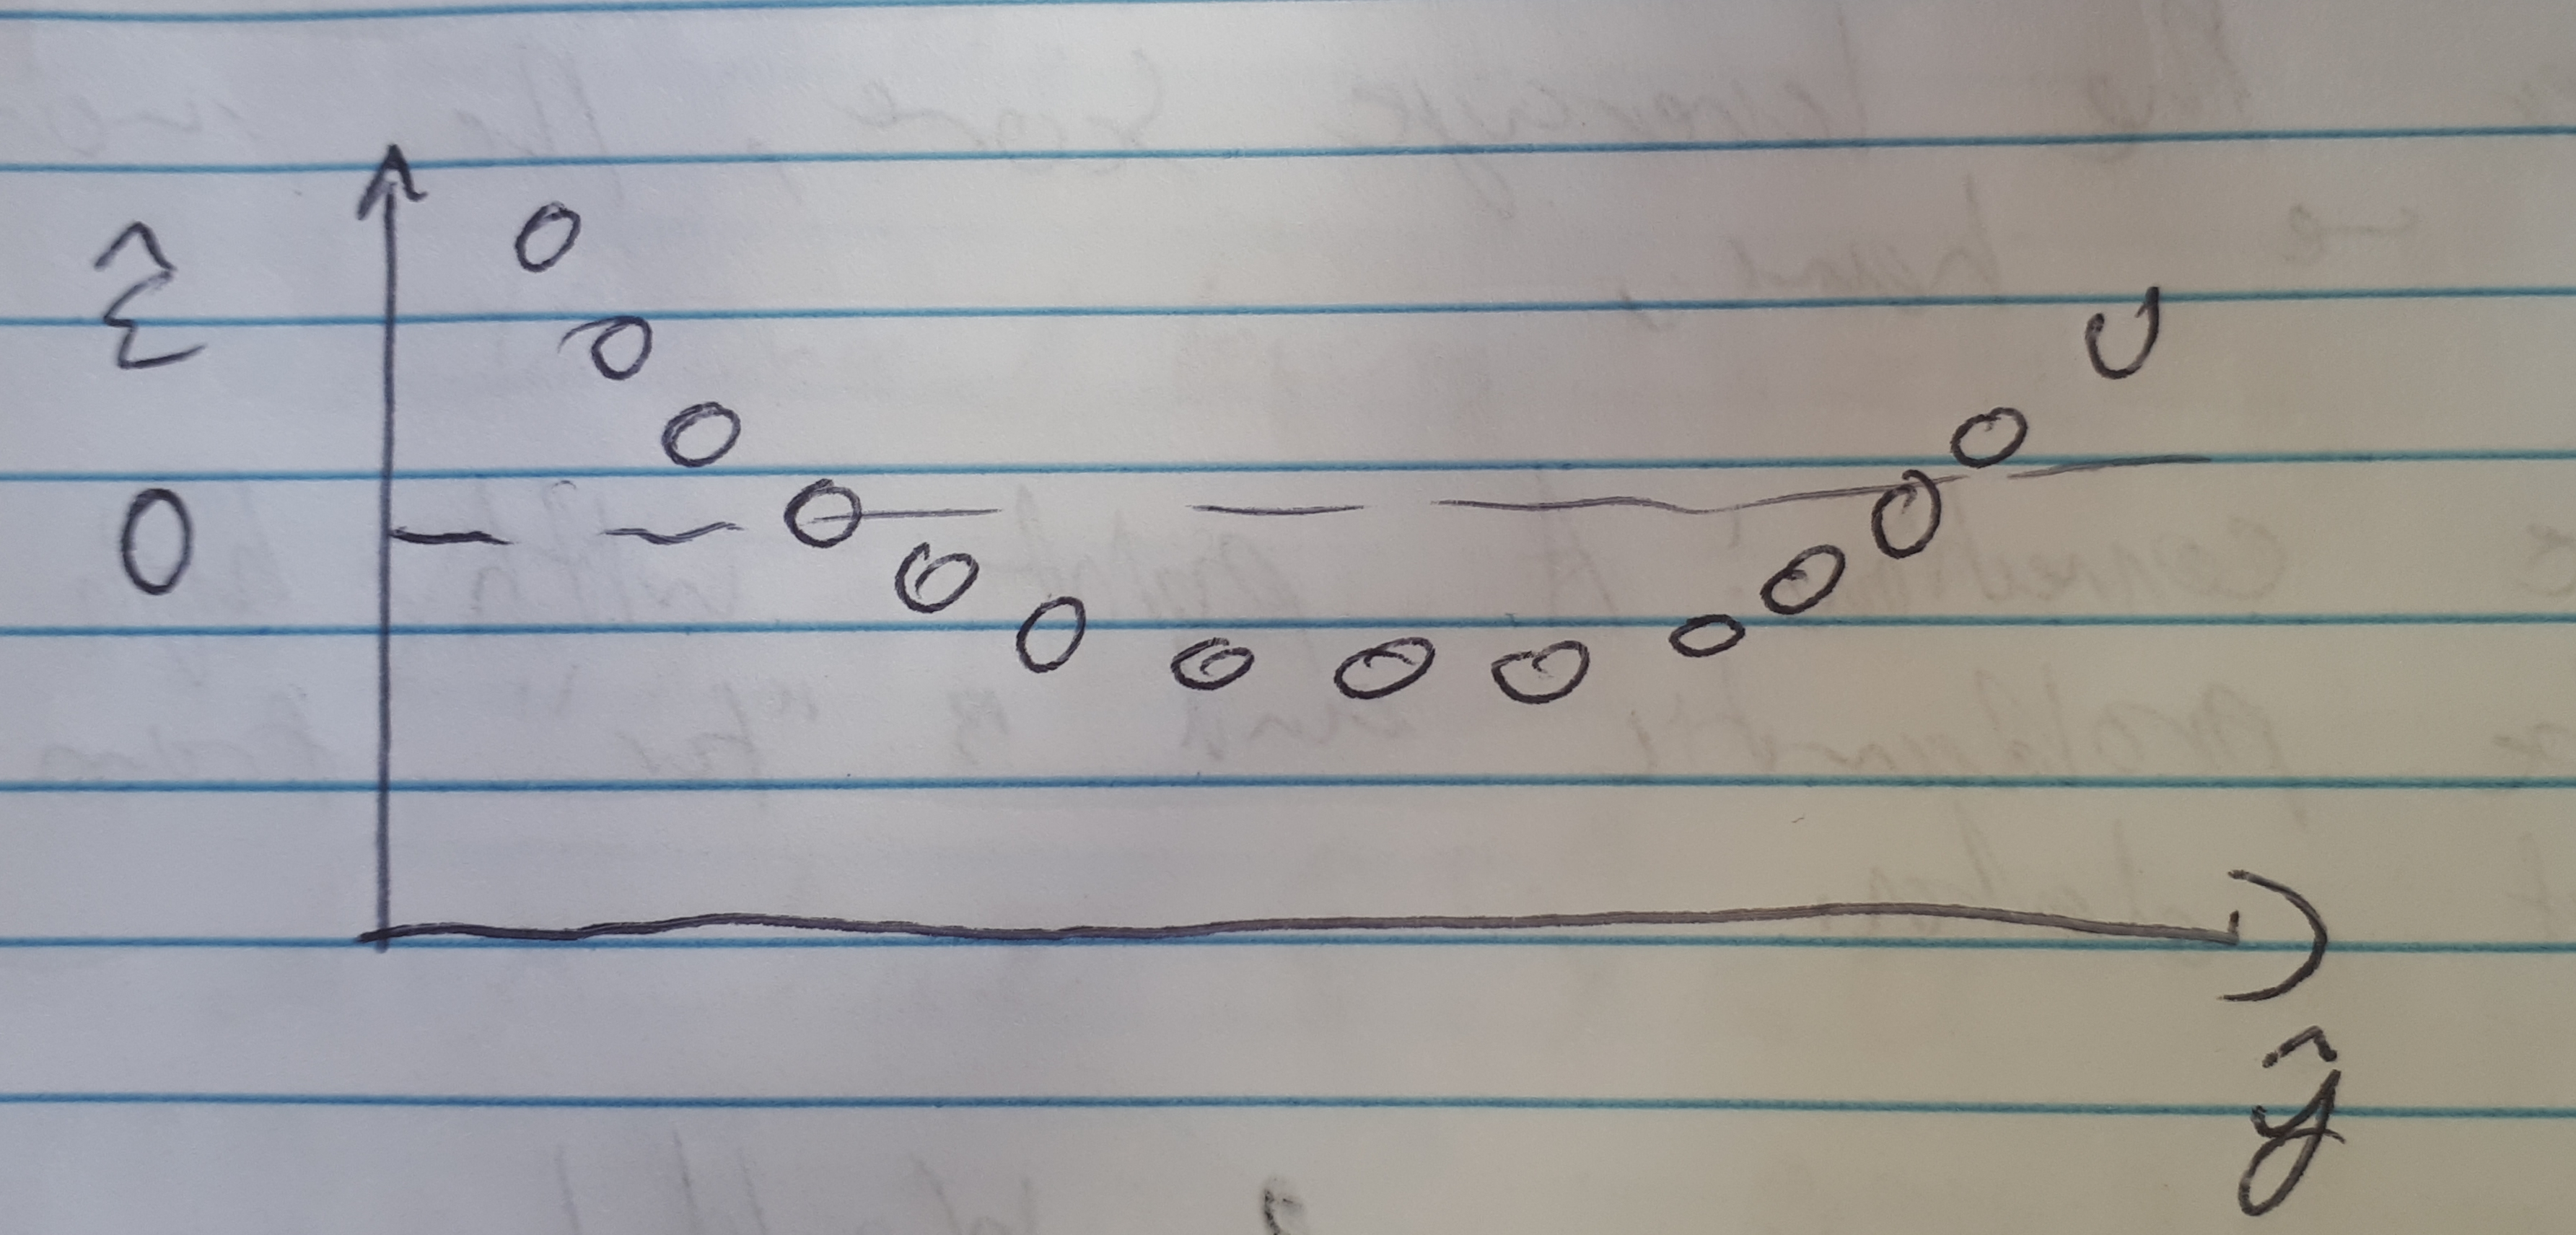
\includegraphics[width = \textwidth/2]{10_26_P02.jpg}
\end{center}

The above data is uncorrelated but there is clear a relationship between $\wh{\eps}$ and $\wh{y}$. You should always plot your residuals against your predicted values to see they are \emph{really} uncorrelated. In the above example we can conclude that the linear model is probably false and we really want to include a term of the form $(x^T\beta)^2$ in our model. Unfortunately this make our model non-linear and there's not much we can do.

The standardized residuals should be roughly Gaussian. That is define
\[\wh{r}_i = \frac{\wh{\eps}_i}{S_n \sqrt{1-H_{ii}}}, \]
where $S_n^2 = \frac{1}{n-d}\norm{X\beta - Y}_2^2 = \frac{1}{n-d}\norm{\wh{\eps}}_2^2$. These normalized residuals should be rouhgly $\Na(0,1)$ at least they should have variance 1. 



\subsection{Residuals vs features}
Suppose $X=[x^{(1)},\ldots, x^{(d)}]$ so $x^{(j)} \in \R^n$ is an individual feature. We could plot the residuals against the individual features.  We might get a plot like this:

\begin{center}
    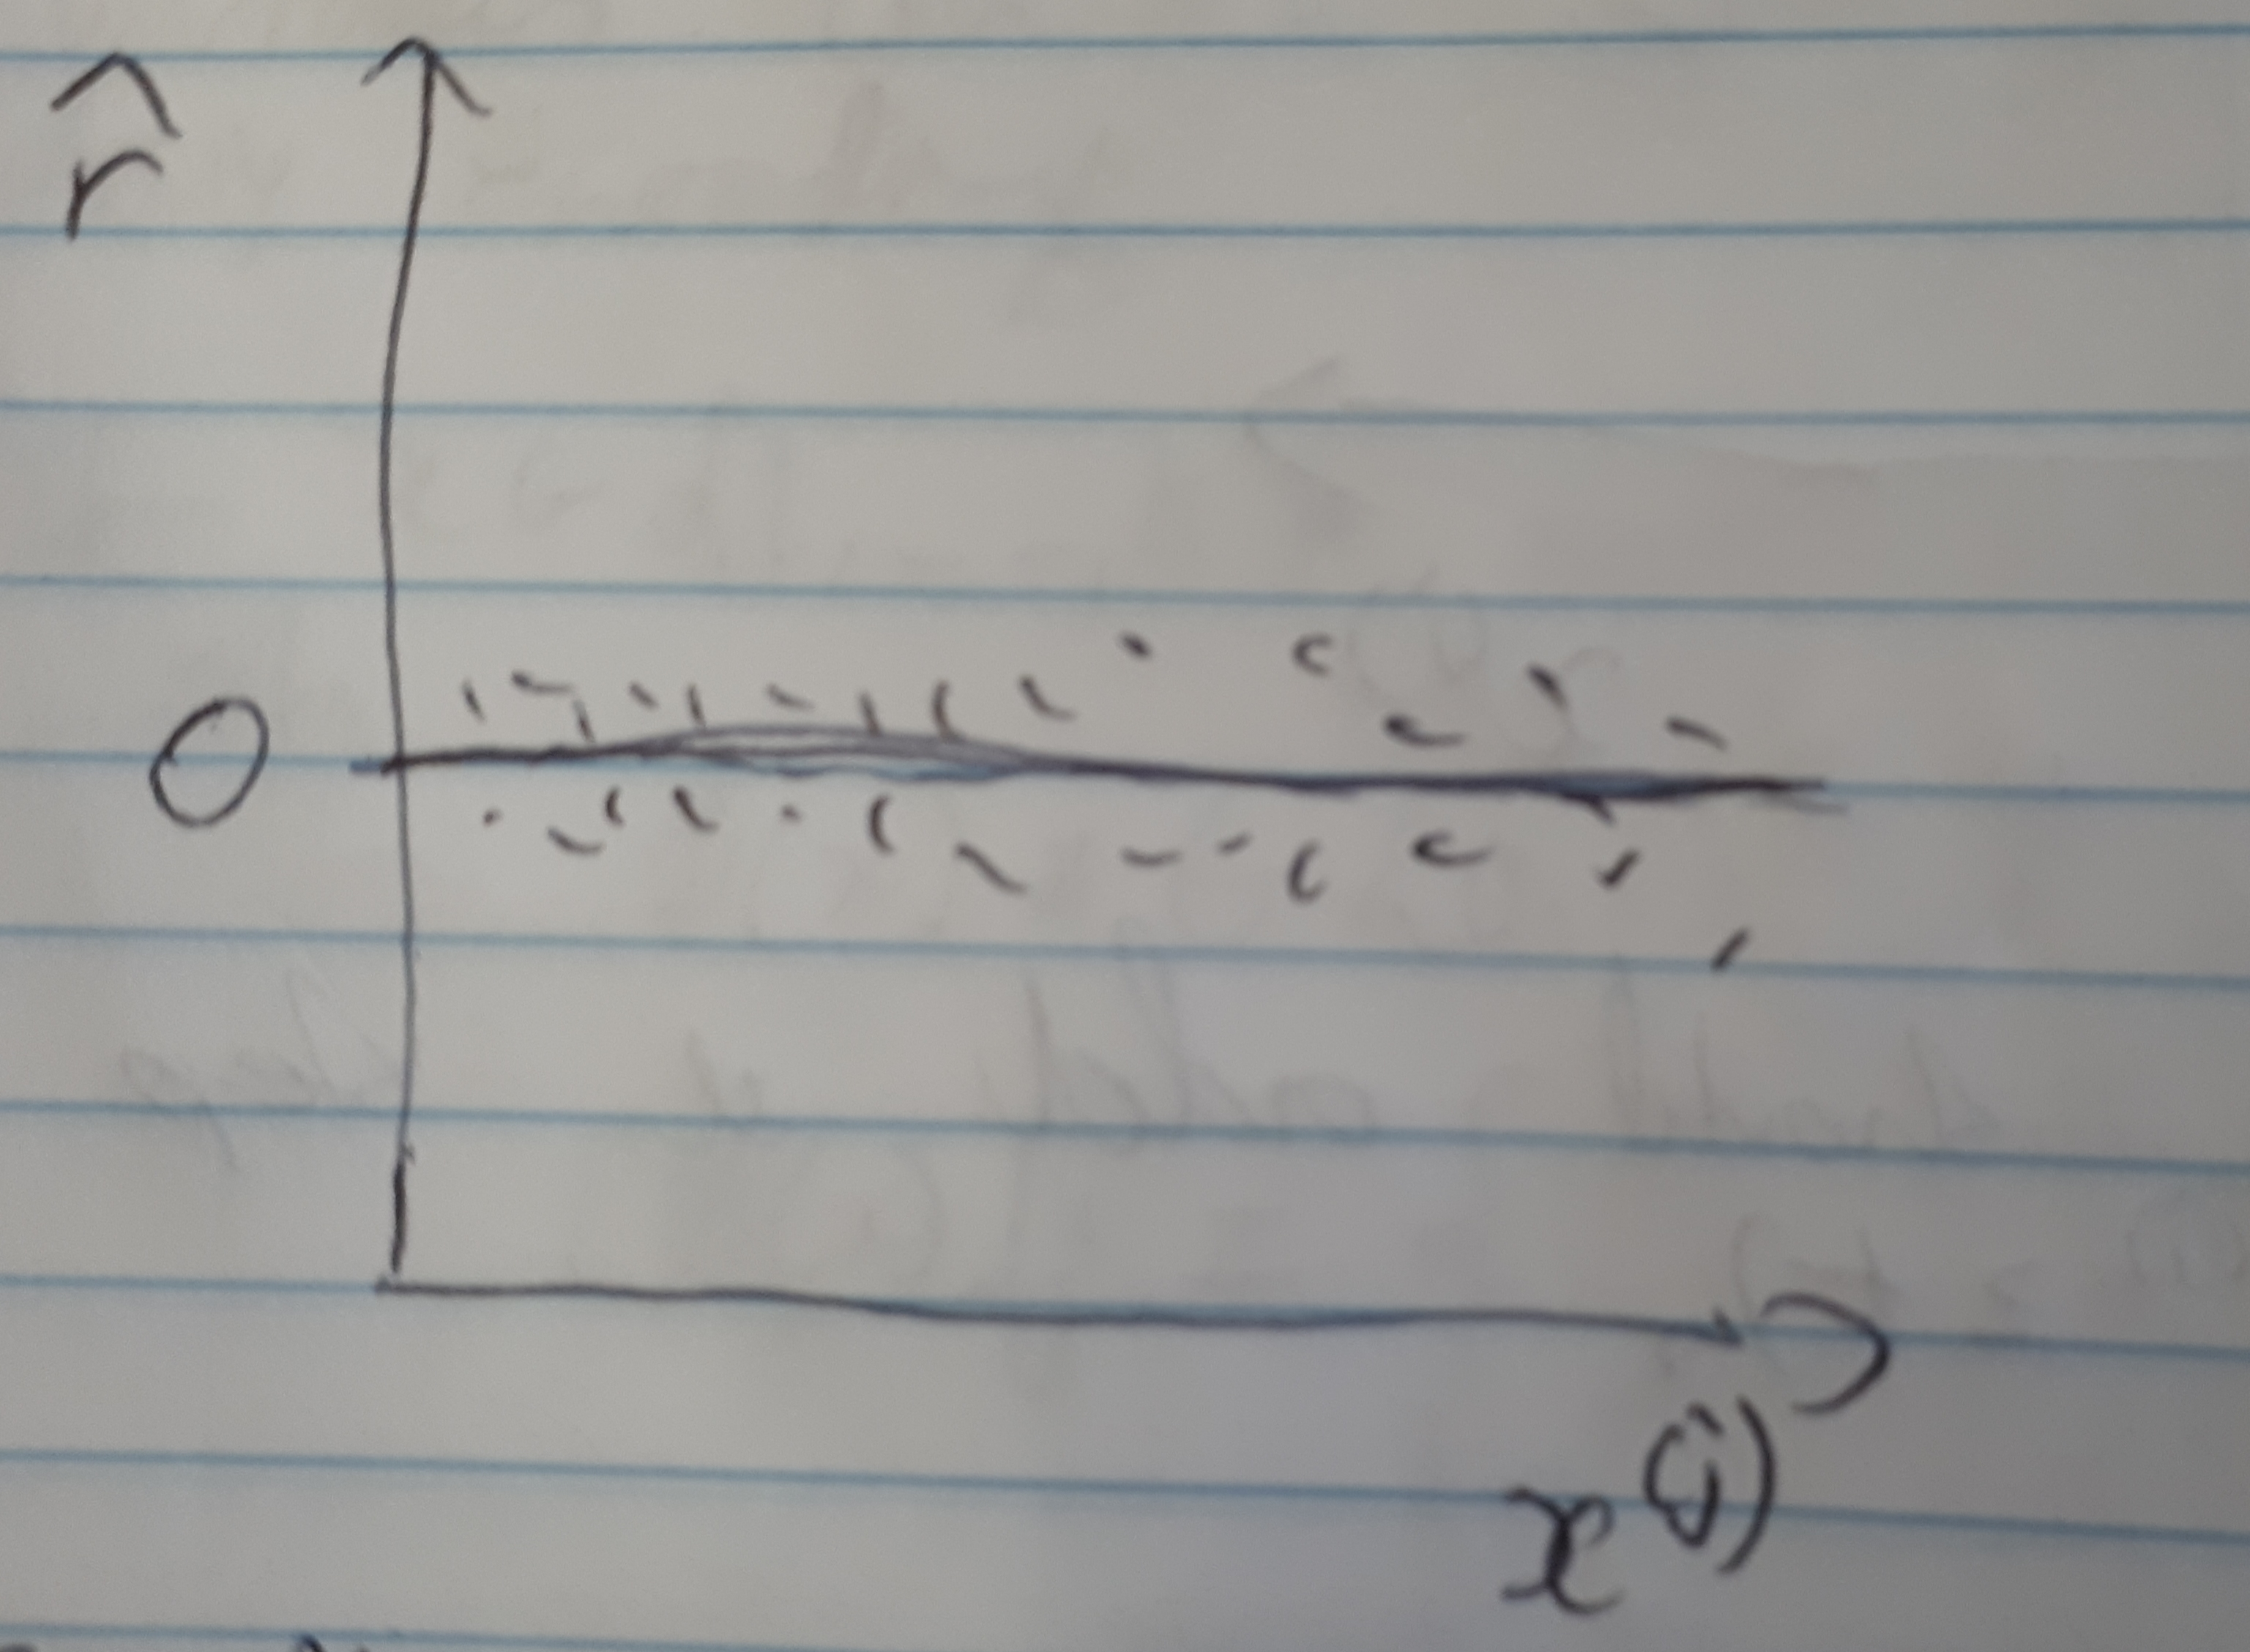
\includegraphics[width = \textwidth/2]{10_26_P03.jpg}
\end{center}

In this situation we are happy and the relationship between the residuals and the feature looks good. We might also have:

\begin{center}
    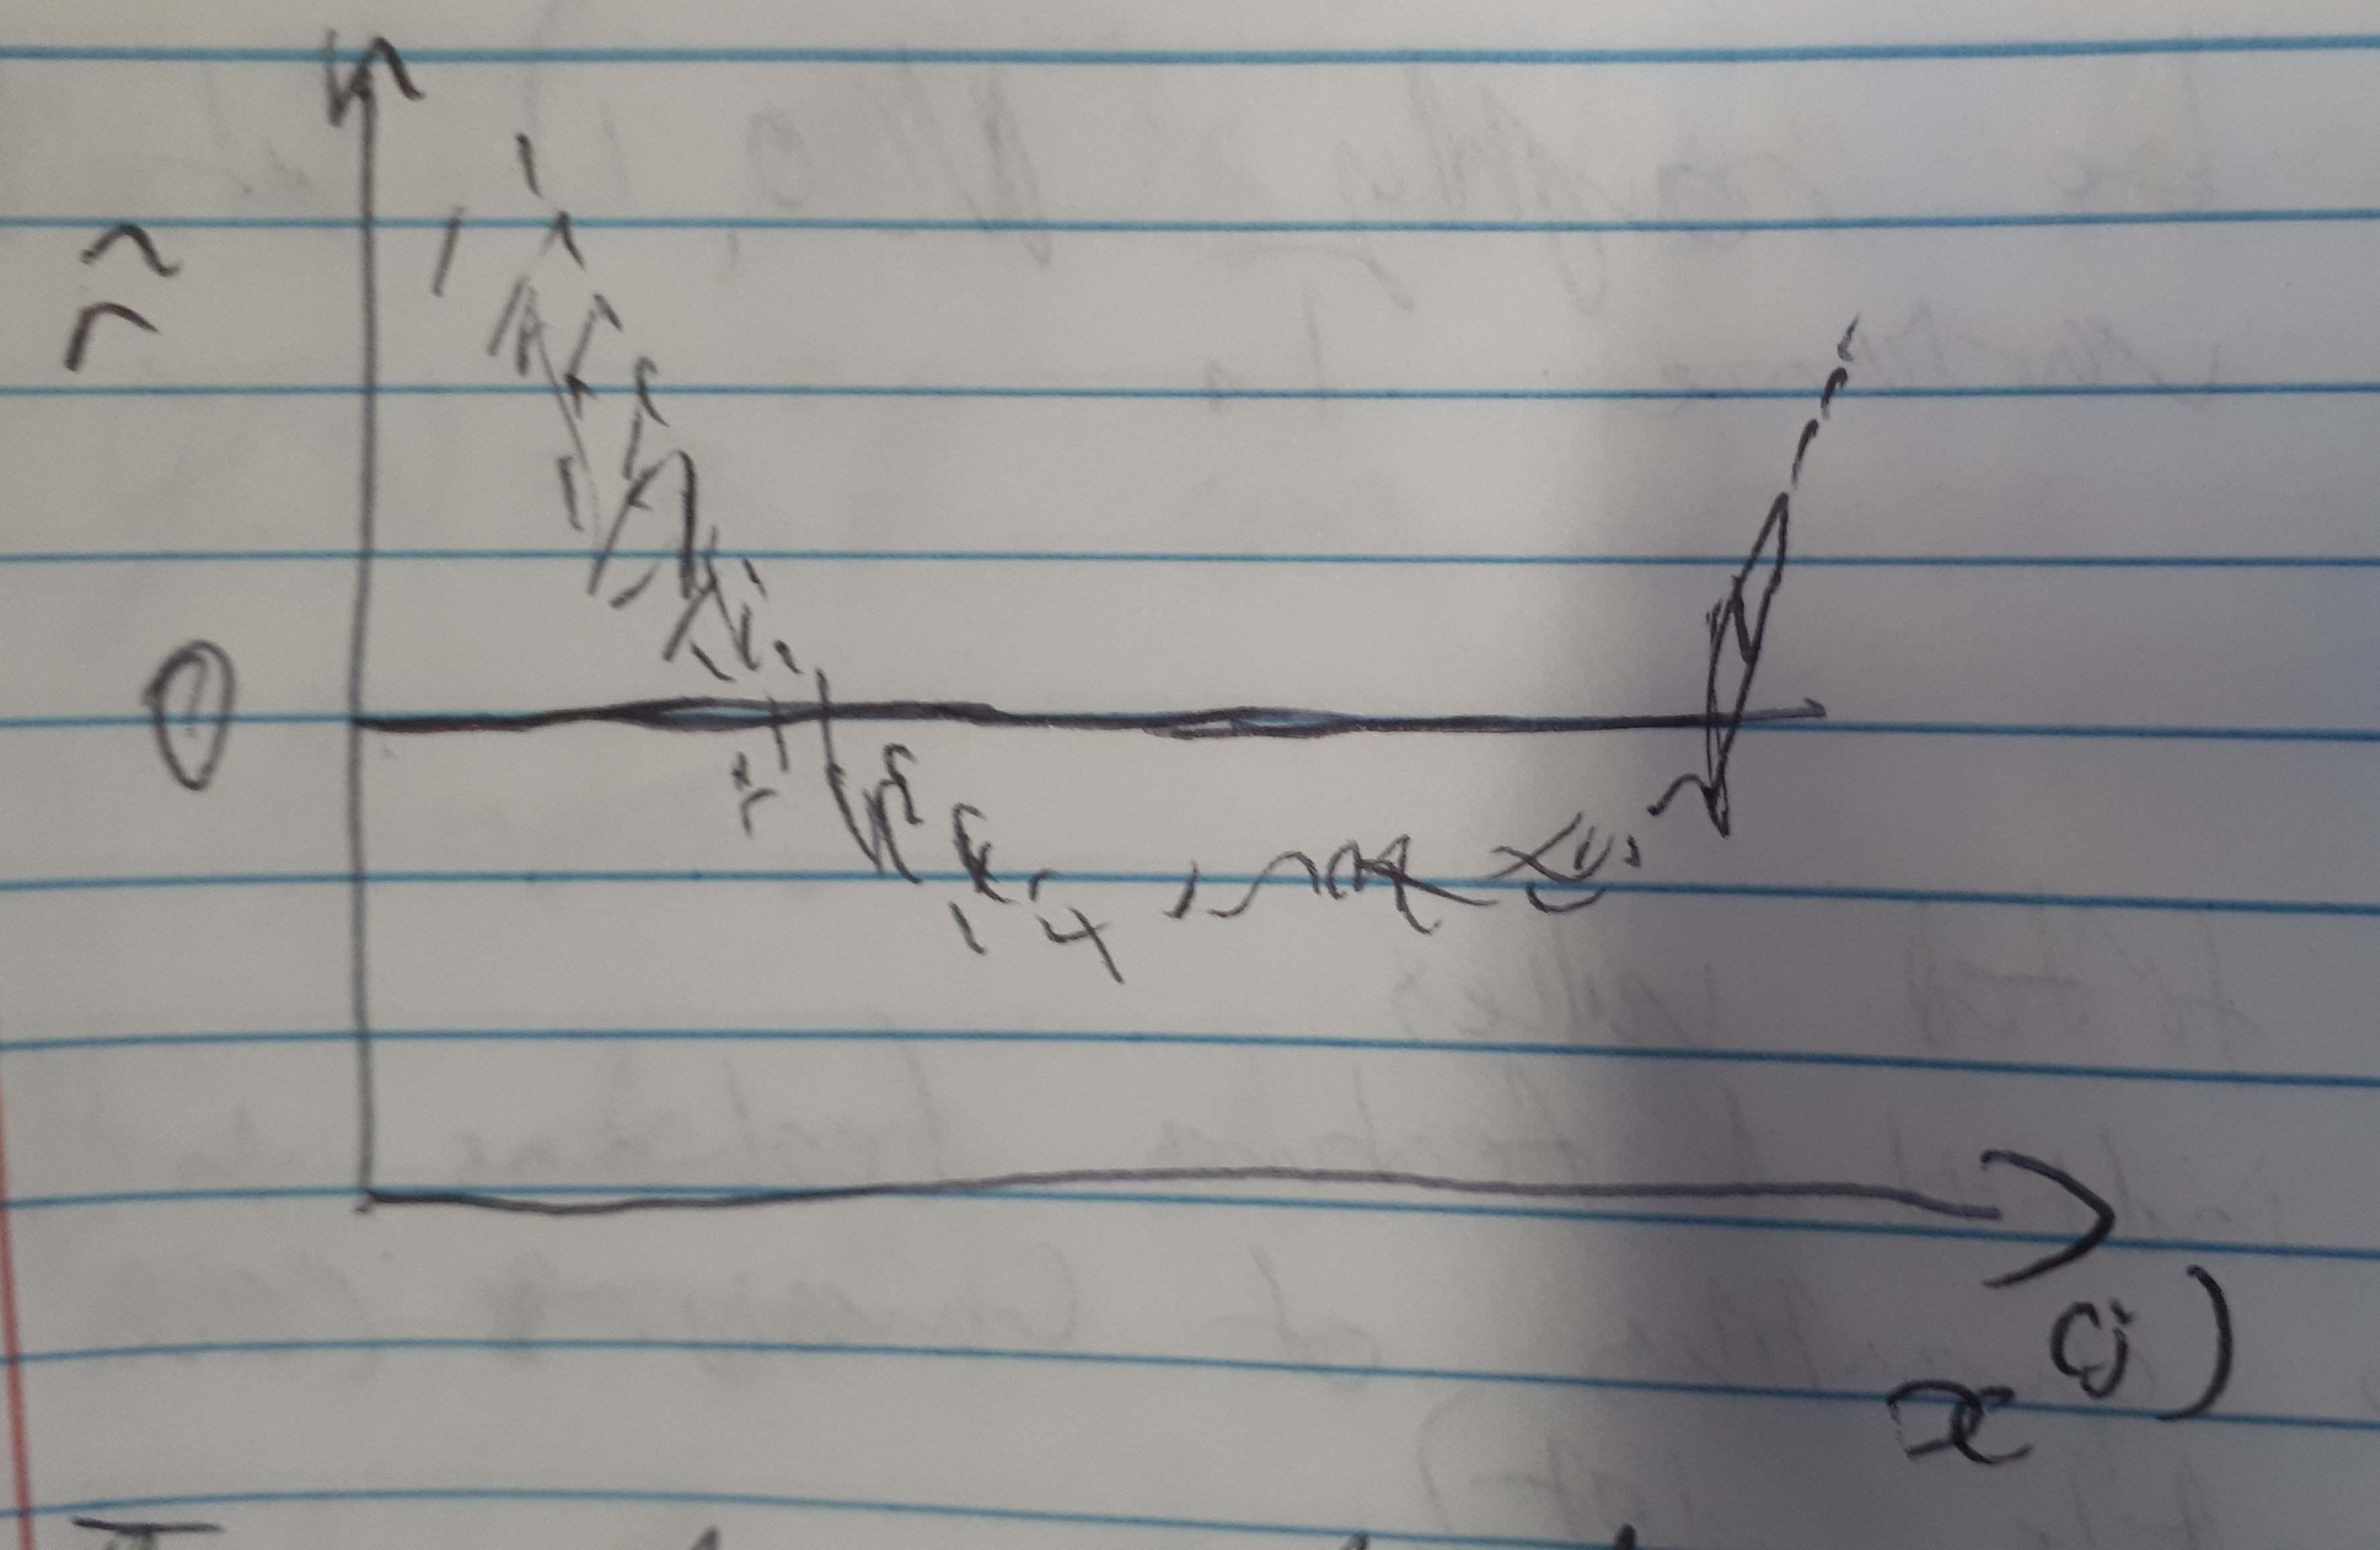
\includegraphics[width = \textwidth/2]{10_26_P04.jpg}    
\end{center}

This suggest we should add a polynomial feature like $(x^{(j)})^2$ to our model. We might also have

\begin{center}
    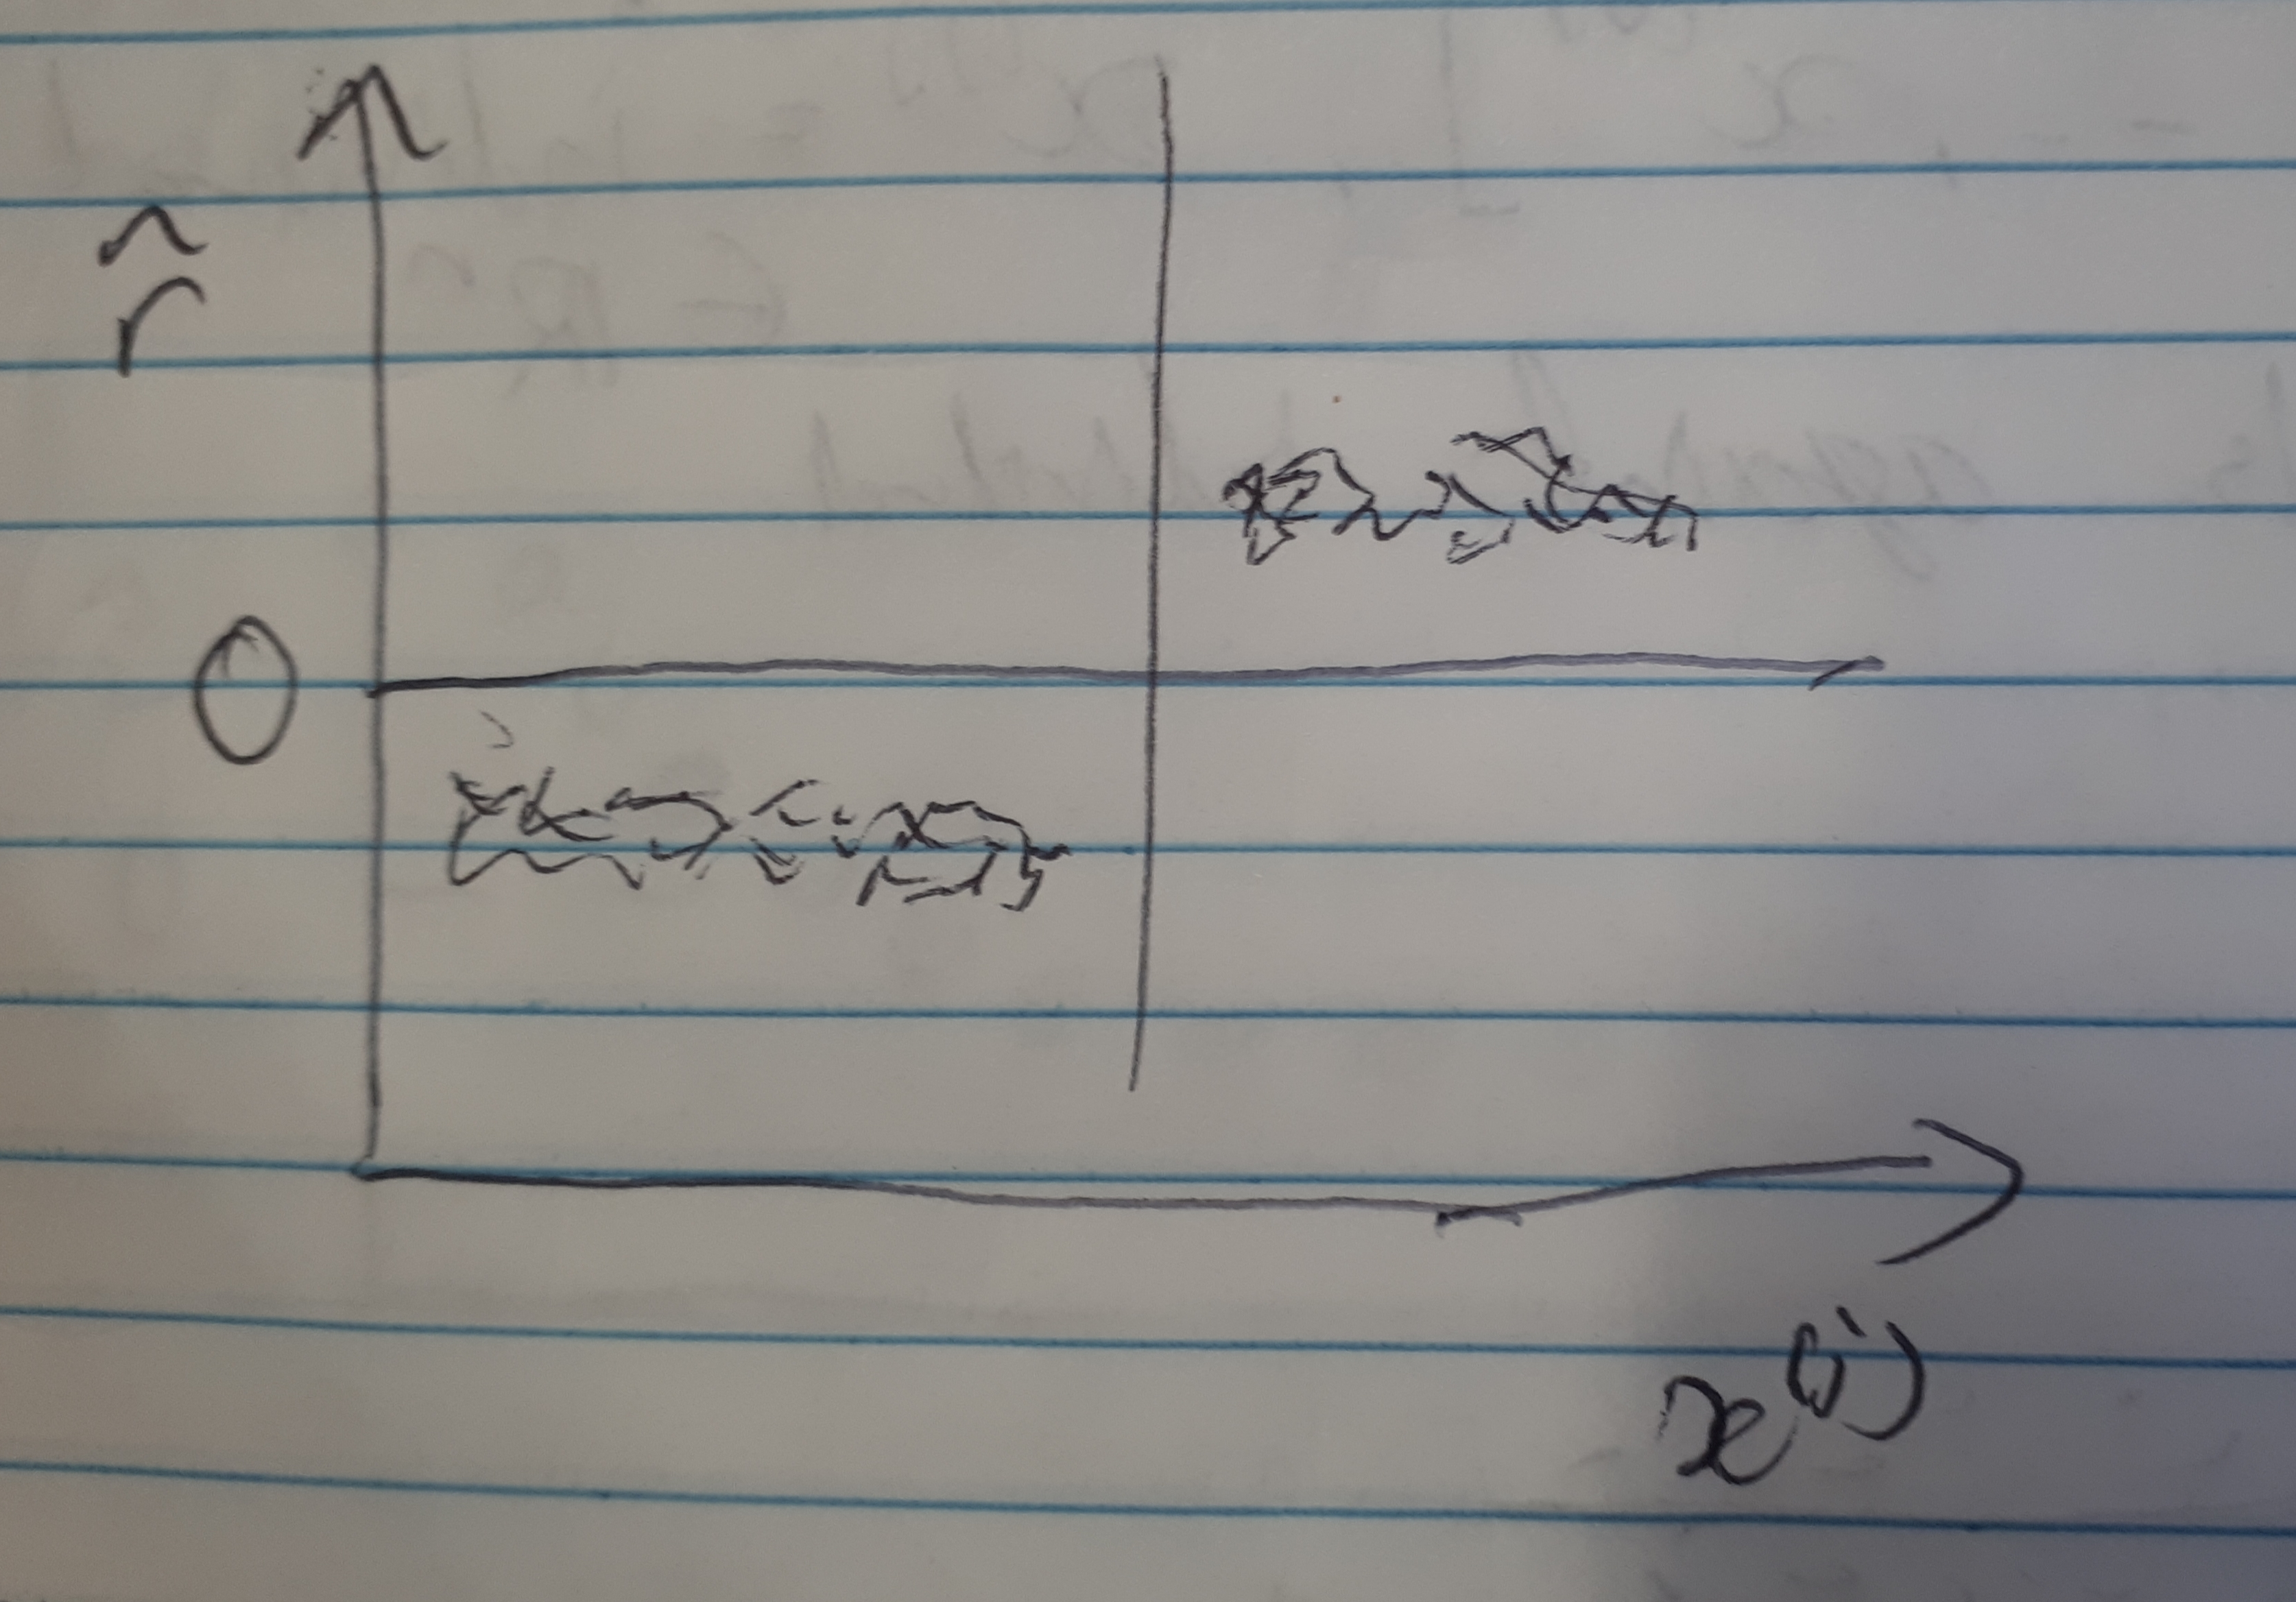
\includegraphics[width = \textwidth/2]{10_26_P05.jpg}
\end{center}

In which case we should add a feature which is a step function like $\one(x^{(j)}>t)$ where $\one(A)$ is the indicator function of $A$. We might have

\begin{center}
    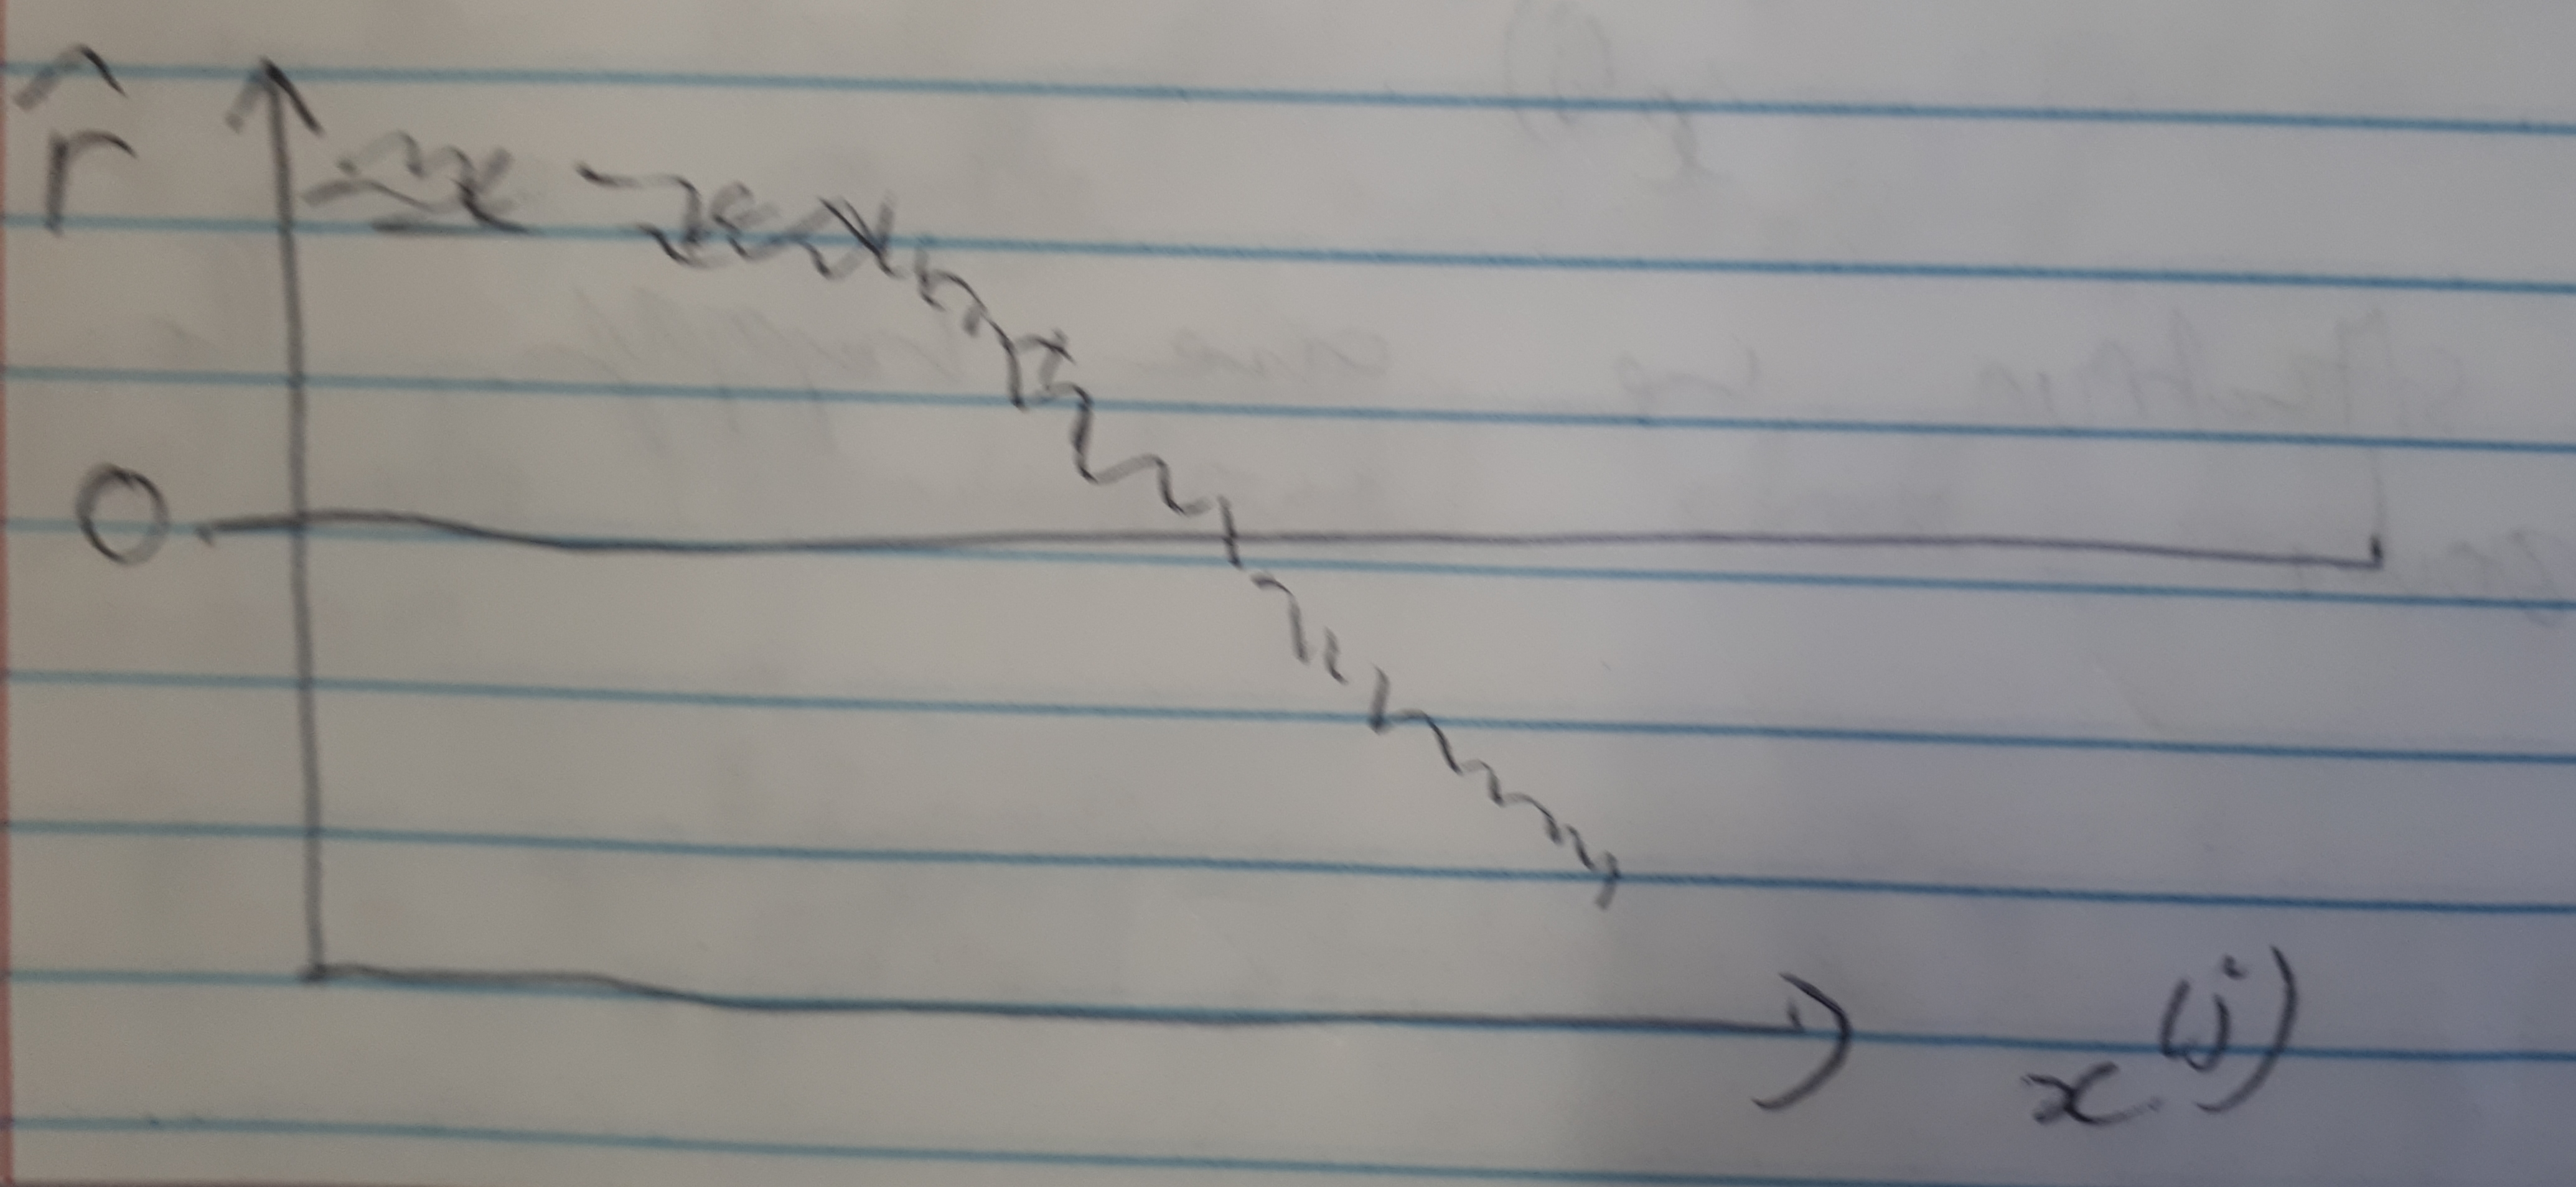
\includegraphics[width = \textwidth/2]{10_26_P06.jpg}
\end{center}

In this case we should add $(x^{(j)}-t)_+$, the positive part of $x^{(j)}-t$. Lastly we might have

\begin{center}
    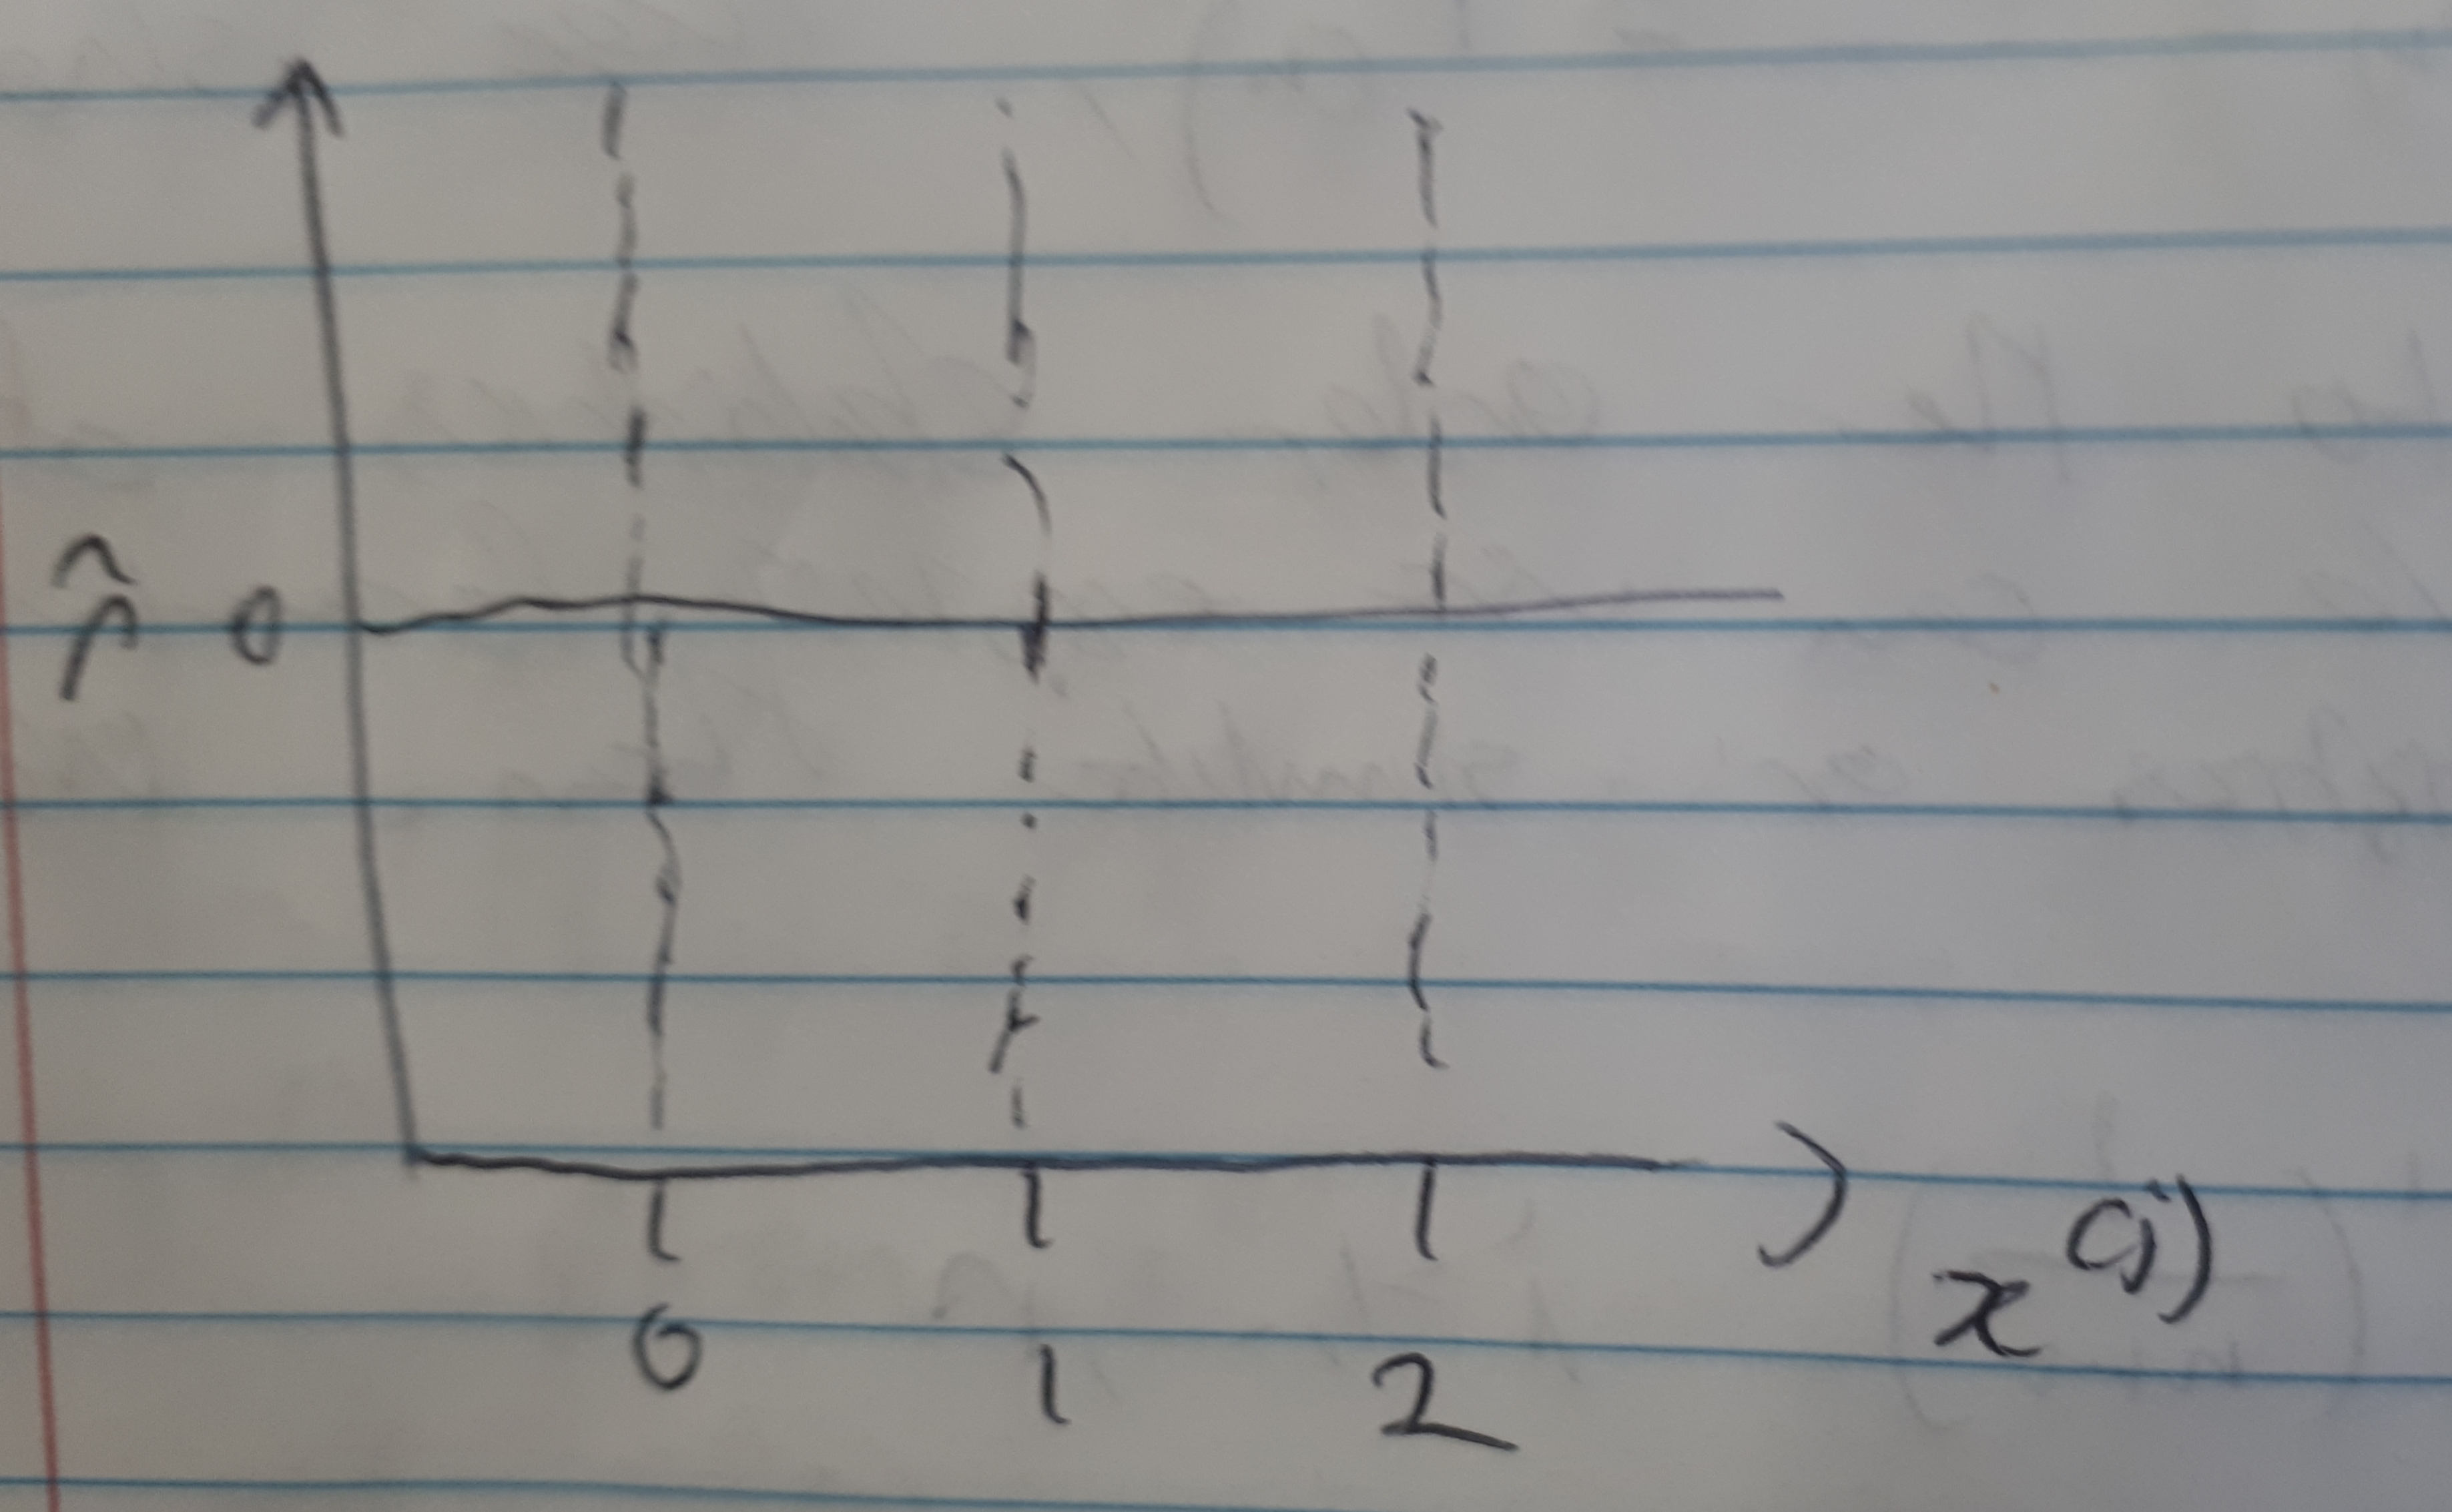
\includegraphics[width = \textwidth/2]{10_26_P07.jpg}
\end{center}

Which means that $x^{(j)}$ is a categorical variable and we should not included it ``raw'' in our model. We should re-encode the variable. There are many names for this re-encoding such as one-hot encoding, dummy variables, factors, $\{0,1\}$-encoding. These all refer to the same process:

If $x \in \{1,\ldots,k\}$, we replace $x$ with $\phi(x)\in \{0,1\}^k$ given by 
\[[\phi(x)]_j = \begin{cases}
    1 & \text{if } x=j,\\
    0&\text{else.}
\end{cases} \]
This is similiar to the encoding used for $k$-groups ANOVA.

\subsection{QQ Plots}
Idea: We can compare the quantiles of $\wh{r}_i = \frac{\wh{\eps}_i}{S_n\sqrt{1-H_{ii}}}$ to the quantiles of a standard normal. First we sort the standized residuals $\wh{r}_{(1)} \le \wh{r}_{(2)} \le \ldots \le \wh{r}_{(n)}$, these should be similiar to the order statistics of a Gaussian. We could use analytic formulas for these order statistics or simulate them. In practice we can also use 
\[v_{(i)}=\Phi^{-1}\left(\frac{i}{n+1}\right), ~~\text{for } i = 1,\ldots,n. \]
We would then expect $v_{(i)} \approx \wh{r}_{(i)}$.

\subsection{Added variable plot}
These give us a sense of how much a variable adds to a model when ``adjusting'' for other variables.

The mathematical insight: Suppose $X = [x^{(1)},\ldots, x^{(d)}]$, then the component of $\wh{\beta}_j$ in ordinary least squares is equal to the regression of $y$ on $x^{(j)}$ adjusting for other variables.

By adjusting we mean we first do regression on $x^{(j)}$ using all the other variables then we subtract this and take $\wh{x}^{(j)}$ to be what's left. Then we use $\wh{x}^{(j)}$ to do regression on $y$.

Let's prove this for $\wh{\beta}_d$. Suppose $X = QR$ where $Q \in \R^{n\times d}$ satisfies $Q^TQ = I_d$ and $R\in \R^{d\times d}$ is invertible and upper triangular. Write $Q=[q_1,\ldots,q_d]$. We know from Gram-Schmidt that if
\[\wh{x}^{(d)} = x^{(d)} - \sum_{j=1}^{d-1}q_j\langle q_j,x^{(d)}\rangle = (I_n-Q_{\setminus d}Q_{\setminus d}^T)x^{(d)}, \]
then $\wh{x}^{(d)}$ is orthogonal to $q_j$ for $j< d$. Thus we can think of $\wh{x}^{(d)}$ as what is left from $x^{(d)}$ after taking away the information in the other variables. We can think of $\wh{x}^{(d)}$ as $x^{(d)}$ with the ``best prediction'' of $x^{(d)}$ from $x^{(1)},\ldots x^{(d-1)}$ removed. We say $\wh{x}^{(d)}$ is $x^{(d)}$ \emph{adjusted for} $x^{(1)},\ldots, x^{(d-1)}$.

Recall that $q_d = \frac{\wh{x}^{(d)}}{\norm{\wh{x}^{(d)}}}_2$ and $R_{dd} = \norm{\wh{x}^{(d)}}_2$. Let's solve the normal equations. Note that
\begin{align*}
    X^TX\beta = X^TY & \Longleftrightarrow R^TQ^TQR\beta = R^TQ^TY\\
    &\Longleftrightarrow R\beta = Q^T Y.
\end{align*}
Thus if we look at the $d^{th}$ component, we see that $\wh{\beta}_d$ must solve $R_{dd}\beta_d = q_d^Ty$. Thus \[\wh{\beta}_d =\frac{(\wh{x}^{(d)})^Ty}{\norm{\wh{x}^{(d)}}_2^2}.\] 

Now consider one dimensional linear regression of $y$ on $z \in \R$. We wish to find 
\[\min_{b \in \R} \sum_{i=1}^n (y_i-z_ib)^2. \]
The minimizer $b^*$ satisfies $\sum_{i=1}^n z_iy_i = \left(\sum_{i=1}^n z_i^2\right)b^*$ and so $b^* = \frac{z^Ty}{\norm{z}_2^2}$. 

Upshot: $\wh{\beta}_j$ is the regression of $y$ onto $x^{(j)}$ adjusting for $x^{(k)}$ for all $k \neq j$.This gives us an idea of something to plot. If we wish to see if the variable $j$ should be included in our model we can plot $y$ adjusted for $x^{(k)}$ for $k \neq j$ against $\wh{x}^{(j)}$. We can then look for a strong linear relationship in the plot. If their is a strong relationship we should include $x^{(j)}$.
\end{document}